\section{System Level Design}

\paragraph{}
In order to accomplish all of the tasks necessary for this DAQ, there were several design choices that were made at the system level.
These include decisions about what microcontroller was being used, the type of data that is being stored, the media device that data is being stored on, how other sensor or control nodes will communicate with the DAQ, what on-board sensors are on the DAQ, how or if the DAQ is able to communicate wirelessly, how a user can interface with the DAQ, and how firmware updates can be applied.

\paragraph{}
The first thing considered was how nodes are able to communicate with the DAQ.
The previous solution used CAN communicating at 1 Mbps to collect data from all nodes on the car.
This became a throughput bottleneck as lower priority CAN ids would occasionally be blocked by the high throughput, higher prioirty data.
The robustness of the CAN bus was very nice and allowed for reliable communication between all nodes on the car.
To keep the robustness of CAN and to improve issues related to throughput, CAN FD with an arbitration rate of 1 Mbps and a data rate of 5 Mbps was selected.

\paragraph{}
The next consideration was how data is stored on the DAQ.
The previous DAQ solution utilized the on-board micro SD card reader on the Teensy 3.5 and Teensy 4.1 microcontrollers and stored data in a CSV format.
The mirco SD card worked well with the small form factor, wide amount of resources available, common communication support with SPI or SDIO, and a reasonable amount of storage for 10 hours of data collection.
As a result, a micro

\begin{figure}[H]
	\centering
	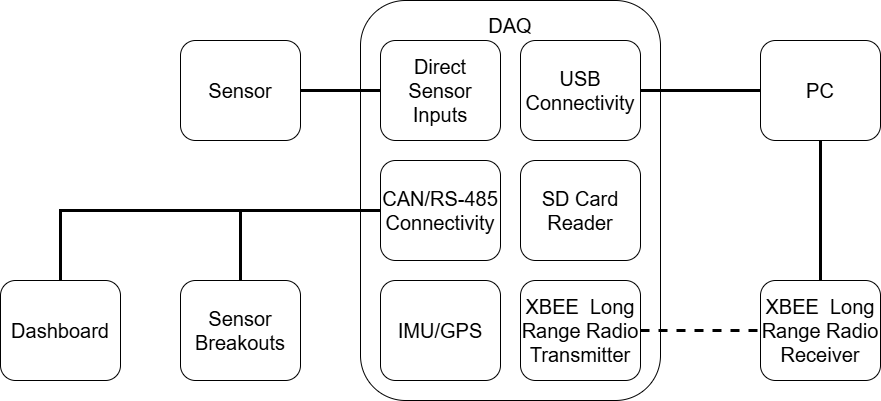
\includegraphics[width=\linewidth]{SystemDiagram.png}
	\caption{System Level Block Diagram}
	\label{fig:SysDiagram}
\end{figure}